\section{Introduction aux composants}
\subsection{Les composants}
Nous avions déjà commencé à aborder les composants : ils permettent de créer des briques d'{\color{monOrange}UI} réutilisables et indépendantes. Nous avions également vu qu'ils étaient organisés de façon hiérarchique en arbre de composants.

Le composant au sommet de l'arbre étant le composant racine ({\color{monOrange}root} en anglais). Ce schéma montre que l'interface utilisateur de gauche est découpée en plusieurs composants : un composant pour l'en-tête, un composant pour la partie principale à gauche et un composant pour la partie droite :

\begin{center}
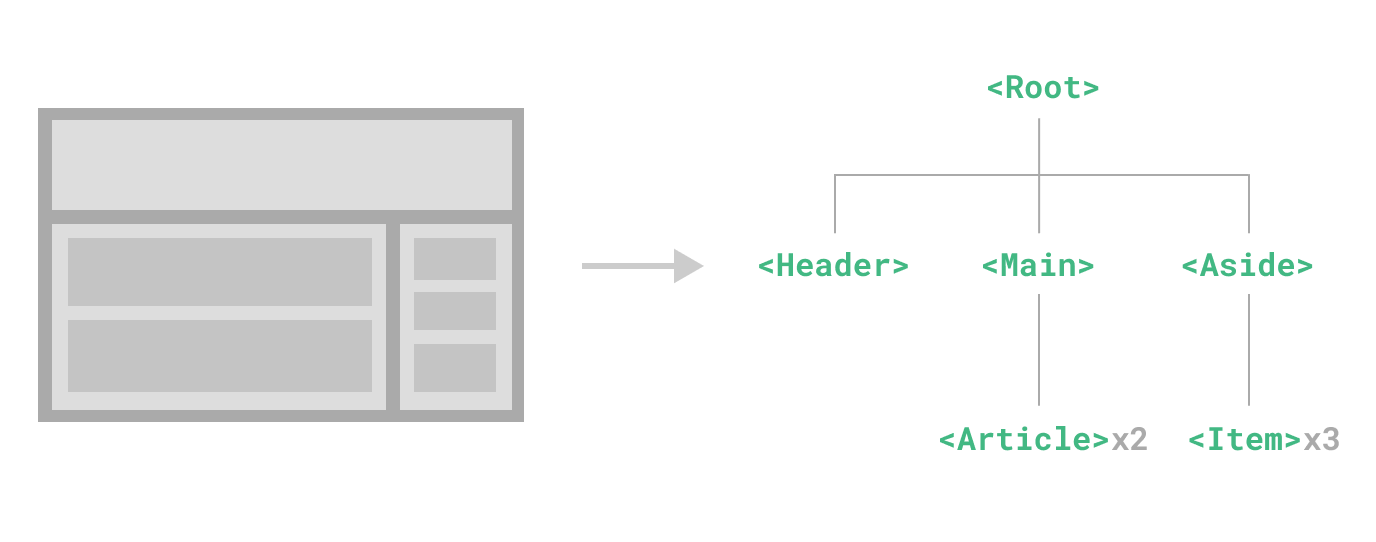
\includegraphics[width=10cm]{images/image08.png}
\end{center}

Remarquez que des composants sont réutilisés plusieurs fois : un composant {\color{monOrange}Article} pour les deux articles affichés et un composant {\color{monOrange}Item} pour les trois informations affichées à droite.

\subsection{Syntaxe des composants}
Nous avons vu que les fichiers des composants étaient écrits en {\color{monOrange}PascalCase} et devaient terminer par l'extension {\color{monOrange}.vue}.

Cette syntaxe permet de créer des composants monofichiers ({\color{monOrange}SFCs}) avec une partie {\color{monOrange}template}, une partie script et une partie style. Cette syntaxe est rendue possible grâce à {\color{monOrange}Vite} et plus précisément au {\color{monOrange}plugin Vue} qui va transformer les {\color{monOrange}SFCs} lors d'une étape de {\color{monOrange}build}.

\subsection{Utiliser des composants enfants}
Pour utiliser un composant enfant dans un composant parent, il suffit d'importer le ou les composants dans la partie {\color{monOrange}script} et de les utiliser dans la partie {\color{monOrange}template}.

La syntaxe recommandée pour utiliser un composant enfant est {\tt <ComposantEnfant />}. Cela permet de distinguer en un coup d'œil les composants {\color{monOrange}Vue.js} des éléments HTML. Dans notre exemple, nous aurions par exemple dans le composant {\color{monOrange}Root }:
\begin{minted}[
mathescape,
framesep=2mm,
baselinestretch=1.2,
%fontsize=\footnotesize,
bgcolor=LightGray,
%linenos
]{html}
<script setup>
import Header from './Header.vue';
import Main from './Main.vue';
import Aside from './Aside.vue';
</script>

<template>
  <Header />
  <Main />
  <Aside />
</template>
\end{minted}
Les composants sont automatiquement exportés grâce à l'utilisation de l'attribut {\color{monOrange}setup} sur les balises {\color{monOrange}scripts}. Aussi, il n'y a rien à exporter manuellement dans les composants enfants.

%Exemple exécutable de la vidéo
%Vous pouvez directement utiliser ce code exécutable. N'hésitez pas à l'ouvrir dans un nouvel onglet pour le modifier ou mieux voir :

\section{Composants locaux et globaux}
\subsection{Enregistrement des composants}
Tous les composants {\color{monOrange}Vue.js} ont besoin d'être enregistrés pour que {\color{monOrange}Vue} puisse savoir où les chercher lorsque vous les utilisez. Il est possible d'enregistrer les composants soit localement, soit globalement.

\subsection{Enregistrement global}
Pour enregistrer des composants globalement, il faut modifier le fichier {\color{monOrange}main.ts} et utiliser la méthode {\color{monOrange}component()} sur l'instance retournée par {\color{monOrange}createApp()} :
\begin{minted}[
mathescape,
framesep=2mm,
baselinestretch=1.2,
%fontsize=\footnotesize,
bgcolor=LightGray,
%linenos
]{javascript}
import { createApp } from 'vue';
import App from './App.vue';
import ComponentA from './'ComponentA'.vue';
import ComponentB from './'ComponentB'.vue';
import ComponentC from './'ComponentC'.vue';


const app = createApp(App);

app
  .component('ComponentA', ComponentA)
  .component('ComponentB', ComponentB)
  .component('ComponentC', ComponentC)

app.mount('#app');
\end{minted}
Le premier argument est le nom à donner au composant dans l'application et le deuxième argument est le composant lui-même qui est importé depuis le fichier où il est situé. Ces composants peuvent être utilisés par n'importe quel composant de votre application, d'où le nom d'enregistrement global. Il existe cependant deux problèmes à l'enregistrement global :
\begin{enumerate}
\item  Le {\color{monOrange}tree-shaking} n'est pas possible. Le {\color{monOrange}tree-shaking} permet d'enlever automatiquement du {\color{monOrange}build} les composants qui ne sont pas utilisés.
\item La relation entre les composants devient difficilement maintenable. Le fait de déclarer tous les composants au même endroit rend difficile le fait de retrouver un composant enfant utilisé dans un composant. Nous n'avons en effet pas accès au chemin dans la partie {\color{monOrange}script} du composant parent. Il faut regarder pour chaque composant dans le fichier {\color{monOrange}main.ts} où il est déclaré. Pour les grandes applications, cela devient rapidement illisible.
\end{enumerate}
\subsection{Enregistrement local}
Les composants enregistrés localement sont disponibles uniquement dans le composant qui les importe. Il est donc nécessaire d'importer le même composant enfant dans tous les composants parents qui l'utilisent. Mais c'est beaucoup plus clair de cette manière : vous savez en un coup d'œil quels composants enfants sont utilisés par un composant en regardant ses imports.

Avant l'apparition de la syntaxe {\color{monOrange}script setup} dans la version {\color{monOrange}3.2}, les composants enregistrés localement devaient être enregistrés comme ceci :
\begin{minted}[
mathescape,
framesep=2mm,
baselinestretch=1.2,
%fontsize=\footnotesize,
bgcolor=LightGray,
%linenos
]{javascript}
import ComponentA from './ComponentA.vue'

export default {
  components: {
    ComponentA
  },
  setup() {
    // ...
  }
}
\end{minted}
Aujourd'hui c'est beaucoup plus simple :
\begin{minted}[
mathescape,
framesep=2mm,
baselinestretch=1.2,
%fontsize=\footnotesize,
bgcolor=LightGray,
%linenos
]{html}
<script setup>
import ComponentA from './ComponentA.vue'
</script>
\end{minted}
Le composant est automatiquement enregistré localement !

%Exemple exécutable de la vidéo
%Vous pouvez directement utiliser ce code exécutable. N'hésitez pas à l'ouvrir dans un nouvel onglet pour le modifier ou mieux voir :


\section{Les props}
\subsection{Communications entre les composants}
Nous avons vu dans les chapitres précédents comment utiliser des composants : comment les définir, comment les instancier, comment fonctionne une architecture en arbre de composants monofichiers etc. Mais il reste un problème : comment faire passer des données le long de notre arbre de composants ?

Comment communiquer des données d'un composant parent vers un composant enfant et d'un composant enfant vers un composant parent ? C'est ce que nous allons voir maintenant.

\subsection{Utilisation des attributs {\color{monOrange}props}}
Vous pouvez passer des valeurs dans le sens parent $\to$ enfant en utilisant des {\color{monOrange}props}. Nous allons partir d'un exemple simple pour bien comprendre.

Supposons que nous avons deux composants : {\color{monOrange}Parent.vue} et {\color{monOrange}Enfant.vue}. Voici notre composant {\color{monOrange}Enfant.vue} :
\begin{minted}[
mathescape,
framesep=2mm,
baselinestretch=1.2,
%fontsize=\footnotesize,
bgcolor=LightGray,
%linenos
]{html}
<template>
  <h3>{{ prenom }}</h3>
</template>

<script setup>
const props = defineProps(['prenom']);
console.log(props.prenom);
</script>
\end{minted}
La fonction {\color{monOrange}defineProps()} permet de déclarer les propriétés récupérées sur le composant enfant depuis le composant parent. Ici nous récupérons {\color{monOrange}prenom}. Elles sont directement utilisables sur le {\color{monOrange}template} et nous pouvons les récupérer dans la partie {\color{monOrange}script} en déclarant une variable {\color{monOrange}props}. Dans notre composant {\color{monOrange}Parent.vue} :
\begin{minted}[
mathescape,
framesep=2mm,
baselinestretch=1.2,
%fontsize=\footnotesize,
bgcolor=LightGray,
%linenos
]{html}
<template>
    <Enfant prenom="Paul" />
</template>

<script>
import Enfant from './Enfant.vue';
</script>
\end{minted}
Nous passons de la donnée de manière unidirectionnelle de {\color{monOrange}Parent.vue} vers {\color{monOrange}Enfant.vue}. Pour ce faire, nous utilisons simplement un attribut {\color{monOrange}prenom} et lui donnons pour l'instant une valeur fixe. Nous pouvons définir n'importe quel attribut personnalisé de cette manière, du moment qu'il n'entre pas en collision avec le nom de d'un attribut HTML natif (par exemple {\color{monOrange}style}).

Il ne faut jamais modifier une {\color{monOrange}props} dans un composant enfant. Nous verrons comment passer des données du composant enfant vers le composant parent.

\subsection{Utilisation d'une liaison dynamique}
Nous souhaitons maintenant que les données que nous passons soient liées de manière dynamique. C'est-à-dire que nous voulons que le composant enfant puisse recevoir la nouvelle valeur de l'attribut que nous lui passons depuis le composant parent lorsqu'elle change. Pour ce faire il suffit d'utiliser la directive {\color{monOrange}v-bind} :
\begin{minted}[
mathescape,
framesep=2mm,
baselinestretch=1.2,
%fontsize=\footnotesize,
bgcolor=LightGray,
%linenos
]{html}
<template>
    <Enfant :prenom="prenom" />
</template>

<script>
import Enfant from './Enfant.vue';
import { ref } from 'vue';

const prenom = ref('Jean');
</script>
\end{minted}
Nous définissons une variable réactive sur notre composant parent {\color{monOrange}prenom}. Nous utilisons la directive {\color{monOrange}v-bind} pour lier cette propriété réactive à la {\color{monOrange}prop} passée au composant enfant.

\subsection{Typage des propriétés props}
Nous avons vu que nous pouvions utiliser sur le composant enfant une fonction {\color{monOrange}defineProps()} et lui passer un tableau avec le nom des {\color{monOrange}props} que nous passons depuis le composant parent. Pour plus de sécurité lors du développement, nous pouvons typer les propriétés sur {\color{monOrange}props} afin de définir le type de valeur attendu.

Les types possibles sont {\color{monOrange}String, Number, Boolean, Array, Object, Function, Date} et {\color{monOrange}Symbol}. Par exemple, pour notre attribut {\color{monOrange}prenom} nous souhaitons que ce dernier soit de type {\color{monOrange}String}. Nous allons donc typer la {\color{monOrange}props} en utilisant un objet au lieu d'un tableau dans la fonction {\color{monOrange}defineProps()} sur le composant enfant :
\begin{minted}[
mathescape,
framesep=2mm,
baselinestretch=1.2,
%fontsize=\footnotesize,
bgcolor=LightGray,
%linenos
]{html}
…
const props = defineProps({
  prenom: String,
});
</script>
...
\end{minted}
Si la valeur de {\color{monOrange}prenom} passée n'est pas de type {\color{monOrange}String}, alors {\color{monOrange}Vue} nous affichera un message d'erreur dans la console JavaScript de notre navigateur. En outre, grâce à {\color{monOrange}Volar} et {\color{monOrange}TypeScript} nous aurons l'auto-complétion des {\color{monOrange}props} et le contrôle des types. Vous pouvez également typer une propriété en permettant plusieurs types, par exemple {\color{monOrange}[String, Number]} :
\begin{minted}[
mathescape,
framesep=2mm,
baselinestretch=1.2,
%fontsize=\footnotesize,
bgcolor=LightGray,
%linenos
]{html}
<script>
//…
const props = defineProps({
  prenom: [String, Number],
});
</script>
...
\end{minted}
Dans ce cas, cette propriété pourra être une chaîne de caractères ou un nombre.

\subsubsection{Utilisation d'un objet pour plus d'options de type}
Vous pouvez également utiliser un objet pour accéder à plus d'options de typage et à des validateurs : Vous pouvez rendre un attribut obligatoire avec {\color{monOrange}required} :
\begin{minted}[
mathescape,
framesep=2mm,
baselinestretch=1.2,
%fontsize=\footnotesize,
bgcolor=LightGray,
%linenos
]{html}
<script>
//…
const props = defineProps({
  prenom: {
        type: String,
        required: true
    }
});
</script>
\end{minted}
Vous pouvez attribuer une valeur par défaut à un attribut :
\begin{minted}[
mathescape,
framesep=2mm,
baselinestretch=1.2,
%fontsize=\footnotesize,
bgcolor=LightGray,
%linenos
]{html}
<script>
//…
const props = defineProps({
  prenom: {
        type: String,
        required: true,
        default: 'Jean'
    }
});
</script>
\end{minted}

\subsubsection{Valeur par défaut des propriétés {\color{monOrange}props} de type {\color{monOrange}Object}}
Si vous souhaitez passer un objet comme donnée depuis un composant parent à un composant enfant, vous pouvez utiliser les mêmes fonctionnalités, cependant vous devrez effectuer une adaptation. La raison est toujours la même : les objets et les tableaux sont passés par référence et non par valeur en JavaScript. Il est donc nécessaire d'utiliser des fonctions pour fabriquer de nouveaux objets pour chaque instance. Dans le cas contraire, le même objet serait utilisé pour toutes les instances d'un composant enfant. Il faut donc utiliser une fonction pour définir une valeur par défaut à notre objet :
\begin{minted}[
mathescape,
framesep=2mm,
baselinestretch=1.2,
%fontsize=\footnotesize,
bgcolor=LightGray,
%linenos
]{javascript}
titre: {
      type: Object,
      default() {
        return { title: 'Mon super titre' }
      }
},
\end{minted}

\subsection{Nommage des {\color{monOrange}props}}
Si vos noms de {\color{monOrange}props} sont longs, il est recommandé d'utiliser côté composant parent le {\color{monOrange}kebab-case} :
\begin{minted}[
mathescape,
framesep=2mm,
baselinestretch=1.2,
%fontsize=\footnotesize,
bgcolor=LightGray,
%linenos
]{html}
<Enfant une-longue-prop="test" />
\end{minted}
Côté composant enfant il faut utiliser le {\color{monOrange}camelCase} pour récupérer la {\color{monOrange}prop} :
\begin{minted}[
mathescape,
framesep=2mm,
baselinestretch=1.2,
%fontsize=\footnotesize,
bgcolor=LightGray,
%linenos
]{html}
<script setup lang="ts">
defineProps({
  uneLongueProp: String
})
</script>
\end{minted}

\subsection{Passer des types statiques autres que des chaînes de caractères}
Pour passer des {\color{monOrange}props} statiques autre que des chaînes de caractères, il faut utiliser {\color{monOrange}v-bind} :
\begin{minted}[
mathescape,
framesep=2mm,
baselinestretch=1.2,
%fontsize=\footnotesize,
bgcolor=LightGray,
%linenos
]{html}
<Enfant :nombre="42" :booleen="false" />
\end{minted}
De même pour les tableaux ou les objets :
\begin{minted}[
mathescape,
framesep=2mm,
baselinestretch=1.2,
%fontsize=\footnotesize,
bgcolor=LightGray,
%linenos
]{html}
<Enfant :tableau="[5, 2, 1]" />
\end{minted}

\subsection{Passer un objet de {\color{monOrange}props}}
Si vous avez de nombreuses {\color{monOrange}props} vous pouvez passer un objet en utilisant la notation longue de {\color{monOrange}v-bind} :
\begin{minted}[
mathescape,
framesep=2mm,
baselinestretch=1.2,
%fontsize=\footnotesize,
bgcolor=LightGray,
%linenos
]{html}
<script>
const objet = {
  id: 1,
  title: 'Un titre'
};
</script>

<template>
  <Enfant v-bind="objet" />
</template>
\end{minted}

%Exemple exécutable de la vidéo
%Vous pouvez directement utiliser ce code exécutable. N'hésitez pas à l'ouvrir dans un nouvel onglet pour le modifier ou mieux voir :

%%%%%%%%%%%%%%%%%%%%%%%%%%%%%%%%%%%%%%%%%%%%%%%%%%%%%%%%%%%

\section{Validation des props et utilisation de TypeScript}
\subsection{Utilisation des validateurs}
Vous pouvez créer un validateur personnalisé pour la valeur de votre attribut. Celui-ci doit être une fonction prenant en paramètre la valeur de l'attribut et doit tester cette valeur puis retourner un booléen :
\begin{minted}[
mathescape,
framesep=2mm,
baselinestretch=1.2,
%fontsize=\footnotesize,
bgcolor=LightGray,
%linenos
]{javascript}
defineProps({
  title: {
    type: String,
    validator(value) {
      return value.length > 2;
    }
  }
}
\end{minted}

\subsection{Notation raccourcie pour les booléens}
Les {\color{monOrange}props} de type booléen ont une notation raccourcie. Par exemple si vous définissez sur le composant enfant :
\begin{minted}[
mathescape,
framesep=2mm,
baselinestretch=1.2,
%fontsize=\footnotesize,
bgcolor=LightGray,
%linenos
]{javascript}
defineProps({
  available: Boolean
})
\end{minted}
Vous pouvez directement passer le {\color{monOrange}prop} de cette manière côté parent :
\begin{minted}[
mathescape,
framesep=2mm,
baselinestretch=1.2,
%fontsize=\footnotesize,
bgcolor=LightGray,
%linenos
]{html}
<Enfant available />
\end{minted}

\subsection{Les génériques TypeScript}
Les génériques sont une fonctionnalité de {\color{monOrange}TypeScript} permettant une grande flexibilité combinée à une sécurité du typage. Lorsque vous débutez avec {\color{monOrange}TypeScript} vous rencontrez deux travers :
\begin{enumerate}
\item Trop typer en {\color{monOrange}any}. Cela vous donne une grande flexibilité mais vous perdez totalement en sécurité et en autocomplétion.

\item Tout typer correctement sans utiliser de génériques. Cela conférera à votre code la sécurité et l'autocomplétion permise par le typage fort mais vous perdrez en flexibilité, ce qui provoque beaucoup de duplications et de lourdes dans votre code.
\end{enumerate}


En résumé, l'objectif des génériques est de permettre d'utiliser des éléments (fonctions, classes, interfaces etc) qui peuvent fonctionner avec une diversité de types tout en conservant l'utilité de {\color{monOrange}TypeScript}, à savoir la sécurité et l'autocomplétion. Nous allons donner deux exemples de types génériques utilisés nativement.

\subsubsection{Le typage des tableaux}
Nous avons vu comment typer des tableaux pour qu'ils n'acceptent qu'un seul type en faisant :
\begin{minted}[
mathescape,
framesep=2mm,
baselinestretch=1.2,
%fontsize=\footnotesize,
bgcolor=LightGray,
%linenos
]{javascript}
const tableau: string[] = ['Des', 'chaînes', 'de', 'caractères'];
\end{minted}
La notation alternative est :
\begin{minted}[
mathescape,
framesep=2mm,
baselinestretch=1.2,
%fontsize=\footnotesize,
bgcolor=LightGray,
%linenos
]{javascript}
const tableau: Array<string> = ['Des', 'chaînes', 'de', 'caractères'];
\end{minted}
Si vous passez la souris sur {\color{monOrange}Array} vous verrez {\tt interface Array<T>}. Cela signifie que {\color{monOrange}Array} prend en fait un argument appelé {\color{monOrange}T} par convention pour type. L'interface {\tt Array<T>} utilise donc un type générique, nous pouvons passer n'importe quel type comme argument et le tableau devra comporter le type défini. Exemple avec une union de types :
\begin{minted}[
mathescape,
framesep=2mm,
baselinestretch=1.2,
%fontsize=\footnotesize,
bgcolor=LightGray,
%linenos
]{javascript}
const tableau: Array<string | boolean> = ['Des', 'chaînes', 'de', 'caractères', true];
\end{minted}
Autre exemple en utilisant une {\color{monOrange}interface} :
\begin{minted}[
mathescape,
framesep=2mm,
baselinestretch=1.2,
%fontsize=\footnotesize,
bgcolor=LightGray,
%linenos
]{javascript}
interface User {
  name: string;
}

const tableau: Array<User> = [{name: 'Paul'}, {name: 'Jean'}];
\end{minted}
Vous commencez à percevoir l'idée de générique : nous passons en argument n'importe quel type à l'interface {\tt Array<T>}, et {\color{monOrange}TypeScript} nous obligera à le respecter.

\subsubsection{Autre exemple : les promesses}
Prenons un exemple avec une promesse :
\begin{minted}[
mathescape,
framesep=2mm,
baselinestretch=1.2,
%fontsize=\footnotesize,
bgcolor=LightGray,
%linenos
]{javascript}
let condition: boolean;

const promesse = new Promise((resolve, reject) => {
  if (condition) {
    resolve(42)
  } else {
    reject('Erreur');
  }
});
\end{minted}
Dans {\color{monOrange}VS Code}, si vous passez la souris sur la constante, vous aurez {\tt Promise<unknown>}. Ici, {\color{monOrange}TypeScript} utilise également un générique pour typer la valeur remboursée par la promesse. Autrement dit, il utilise une {\tt interface Promise<T>}, et donc les génériques. Ici, il ne peut pas détecter le type par inférence et préciser donc que la valeur retournée est de type inconnu : {\color{monOrange}unknown}. En revanche, si nous passons un argument, {\color{monOrange}TypeScript} saura que les valeurs retournées dans les promesses seront du type spécifié :
\begin{minted}[
mathescape,
framesep=2mm,
baselinestretch=1.2,
%fontsize=\footnotesize,
bgcolor=LightGray,
%linenos
]{javascript}
let condition: boolean;

const promesse: Promise<number | string> = new Promise((resolve, reject) => {
  if (condition) {
    resolve(42)
  } else {
    reject('Erreur');
  }
});
\end{minted}
Ici, nous indiquons à {\color{monOrange}TypeScript} les valeurs retournées dans la promesse ce qui permet la sécurité et l'autocomplétion. A savoir que si vous essayez d'utiliser par exemple une méthode disponible sur les tableaux ou les objets sur la valeur de retour, {\color{monOrange}TypeScript} vous renverra une erreur. Par exemple :
\begin{minted}[
mathescape,
framesep=2mm,
baselinestretch=1.2,
%fontsize=\footnotesize,
bgcolor=LightGray,
%linenos
]{javascript}
let condition: boolean;

const promesse: Promise<number | string> = new Promise((resolve, reject) => {
  if (condition) {
    resolve(42)
  } else {
    reject('Erreur');
  }
});

promesse.then((val) => {
  val.map()
})
\end{minted}
Ici, vous aurez une erreur {\color{red}Property 'map' does not exist on type 'string | number'}.

De même, {\color{monOrange}VS Code} vous proposera en autocomplétion sur {\color{monOrange}val} les méthodes et propriétés partagées par les types nombre et chaînes de caractères. Si vous mettiez {\tt Promise<any>}, {\color{monOrange}TypeScript} ne feriez plus de contrôle sur les valeurs de retour, sur les méthodes que l'on tente d'accéder etc.
\begin{minted}[
mathescape,
framesep=2mm,
baselinestretch=1.2,
%fontsize=\footnotesize,
bgcolor=LightGray,
%linenos
]{javascript}
let condition: boolean;

const promesse: Promise<any> = new Promise((resolve, reject) => {
  if (condition) {
    resolve(42)
  } else {
    reject('Erreur');
  }
});

promesse.then((val) => {
  val.map()
})
\end{minted}
Ici aucun problème lors de la compilation et dans {\color{monOrange}VS Code}, pourtant l'accès à la méthode {\color{monOrange}map()} provoquera une erreur lors de l' ;exécution.

\subsection{Utilisation de {\color{monOrange}TypeScript} avec les {\color{monOrange}props}}
Vous pouvez également utiliser la syntaxe {\color{monOrange}TypeScript} au lieu de passer un objet à {\color{monOrange}props}, dans ce cas on utilise un type générique
\begin{minted}[
mathescape,
framesep=2mm,
baselinestretch=1.2,
%fontsize=\footnotesize,
bgcolor=LightGray,
%linenos
]{html}
<script setup lang="ts">
defineProps<{
  prenom?: string
  age?: number
}>()
</script>
\end{minted}
Remarquez que nous utilisons un type générique et non plus un argument passé à {\color{monOrange}defineProps()}. Le plus souvent nous utiliserons des {\color{monOrange}interfaces} de cette manière ;
\begin{minted}[
mathescape,
framesep=2mm,
baselinestretch=1.2,
%fontsize=\footnotesize,
bgcolor=LightGray,
%linenos
]{html}
<script setup lang="ts">
interface Props {
  prenom: string
  age?: number
}

const props = defineProps<Props>()
</script>
\end{minted}

%Exemple exécutable de la vidéo
%Vous pouvez directement utiliser ce code exécutable. N'hésitez pas à l'ouvrir dans un nouvel onglet pour le modifier ou mieux voir :

%%%%%%%%%%%%%%%%%%%%%%%%%%%%%%%%%%%%%%%%%%%%%%%%%%%%%%%%%%%%%%

\section{Les événements}
\subsection{Communiquer des composants enfants vers les composants parents}
Nous allons maintenant nous intéresser au sens de communication inverse : des composants enfants vers les composants parents. Pour communiquer dans ce sens, nous utilisons les événements personnalisés. Il faut déclarer l'événement sur le composant enfant et l'écouter sur le composant parent. Dans le {\color{monOrange}template} du composant parent, nous enregistrons l'écoute d'un événement personnalisé avec la directive {\color{monOrange}v-on} :
\begin{minted}[
mathescape,
framesep=2mm,
baselinestretch=1.2,
%fontsize=\footnotesize,
bgcolor=LightGray,
%linenos
]{javascript}
<Enfant
  ...
  @un-evenement="gestionnaire"
 />
\end{minted}
Dans la partie {\color{monOrange}script} du composant enfant, nous déclarons l'événement avec {\color{monOrange}defineEmits()} :
\begin{minted}[
mathescape,
framesep=2mm,
baselinestretch=1.2,
%fontsize=\footnotesize,
bgcolor=LightGray,
%linenos
]{javascript}
const emit = defineEmits(['un-evenement']);
\end{minted}
Nous pouvons émettre l'événement côté {\color{monOrange}script} en utilisant :
\begin{minted}[
mathescape,
framesep=2mm,
baselinestretch=1.2,
%fontsize=\footnotesize,
bgcolor=LightGray,
%linenos
]{javascript}
emit('un-evenement');
\end{minted}

\subsection{Émettre des événements sans utiliser defineEmits()}
Côté composant enfant, vous pouvez émettre directement des événements sans passer par {\color{monOrange}defineEmits()}, en utilisant {\tt \$emit()} dans le {\color{monOrange}template} :
\begin{minted}[
mathescape,
framesep=2mm,
baselinestretch=1.2,
%fontsize=\footnotesize,
bgcolor=LightGray,
%linenos
]{html}
<button @click="$emit('unEvenement')">Cliquer</button>
\end{minted}
Il faut utiliser le {\color{monOrange}camelCase} pour le nom de l'événement. Côté composant, parent, cela ne change pas, nous utilisons {\color{monOrange}v-on} pour écouter l'événement écrit en {\color{monOrange}kebab-case} :
\begin{minted}[
mathescape,
framesep=2mm,
baselinestretch=1.2,
%fontsize=\footnotesize,
bgcolor=LightGray,
%linenos
]{html}
<Enfant @un-evenement="gestionnaire" />
\end{minted}
\subsection{Passer des arguments}
Vous pouvez passer des arguments lors de l'émission d'un événement. Il suffit de les passer en argument dans le composant enfant :
\begin{minted}[
mathescape,
framesep=2mm,
baselinestretch=1.2,
%fontsize=\footnotesize,
bgcolor=LightGray,
%linenos
]{html}
<button @click="$emit('unEvenement', 42, 'unEvenement')">Cliquer</button>
\end{minted}
Côté composant parent vous pouvez les récupérer dans le gestionnaire d'événement :
\begin{minted}[
mathescape,
framesep=2mm,
baselinestretch=1.2,
%fontsize=\footnotesize,
bgcolor=LightGray,
%linenos
]{html}
<Enfant @un-evenement="gestionnaire" />
\end{minted}
Par exemple :
\begin{minted}[
mathescape,
framesep=2mm,
baselinestretch=1.2,
%fontsize=\footnotesize,
bgcolor=LightGray,
%linenos
]{javascript}
function gestionnaire(arg1, arg2) {
  console.log(arg1, arg2);
}
\end{minted}

\subsection{Validation des évenements}
Comme pour les {\color{monOrange}props}, il est possible de valider les événements, même si c'est assez peu utilisé. Par exemple :
\begin{minted}[
mathescape,
framesep=2mm,
baselinestretch=1.2,
%fontsize=\footnotesize,
bgcolor=LightGray,
%linenos
]{html}
<script setup>
const emit = defineEmits({
  submit: ({ email, password }) => {
    if (email && password) {
      return true;
    } else {
      return false;
    }
  }
})

function submitForm(email, password) {
  emit('submit', { email, password })
}
</script>
\end{minted}
Ici notre événement {\color{monOrange}submit} prend en argument un objet  {\color{monOrange}\{ email, password \}}. La fonction de validation définie dans {\color{monOrange}defineEmits()} reçoit cet argument dans une fonction de rappel. Cette fonction de rappel retourne {\color{monOrange}true} si l'événement est valide et false sinon. Ici, il est considéré que l'événement est valide si {\color{monOrange}email} et {\color{monOrange}password} sont définis.

{\em Nous ne détaillerons pas davantage car ce type de validation est très rarement utilisé, et seulement en développement. Nous verrons comment valider des formulaires plus tard}.

\subsection{Syntaxe recommandée : utilisation de {\color{monOrange}defineEmits} avec {\color{monOrange}TypeScript}}
Dans la suite de la formation nous utiliserons ce qui est recommandé par {\color{monOrange}Vue} officiellement : déclarer explicitement les événements utilisés avec {\color{monOrange}defineEmits()} en utilisant {\color{monOrange}TypeScript}. Comme pour les {\color{monOrange}props}, il suffit de passer un générique à la fonction pour déclarer les types des événements utilisés :
\begin{minted}[
mathescape,
framesep=2mm,
baselinestretch=1.2,
%fontsize=\footnotesize,
bgcolor=LightGray,
%linenos
]{javascript}
const emit = defineEmits<{
  (e: 'change', id: number): void;
  (e: 'update', value: string): void;
}>()
\end{minted}

Ici nous déclarons un événement {\color{monOrange}change} qui contient un argument {\color{monOrange}id} de type {\color{monOrange}number} et un événement {\color{monOrange}update} qui contient un argument {\color{monOrange}value} de type chaîne de caractères.

%Exemple exécutable de la vidéo
%Vous pouvez directement utiliser ce code exécutable. N'hésitez pas à l'ouvrir dans un %nouvel onglet pour le modifier ou mieux voir :

%%%%%%%%%%%%%%%%%%%%%%%%%%%%%%%%%%%%%%%%%%%%%%%%%%%%%%

\section{Le cycle de vie d'un composant}
\subsection{Le cycle de vie des composants}
Les composants {\color{monOrange}Vue.js} passent par différents stades de leur initialisation, à l'affichage sur le DOM, puis à leurs mises à jour et enfin à leur destruction et enlèvement du DOM.
\begin{center}
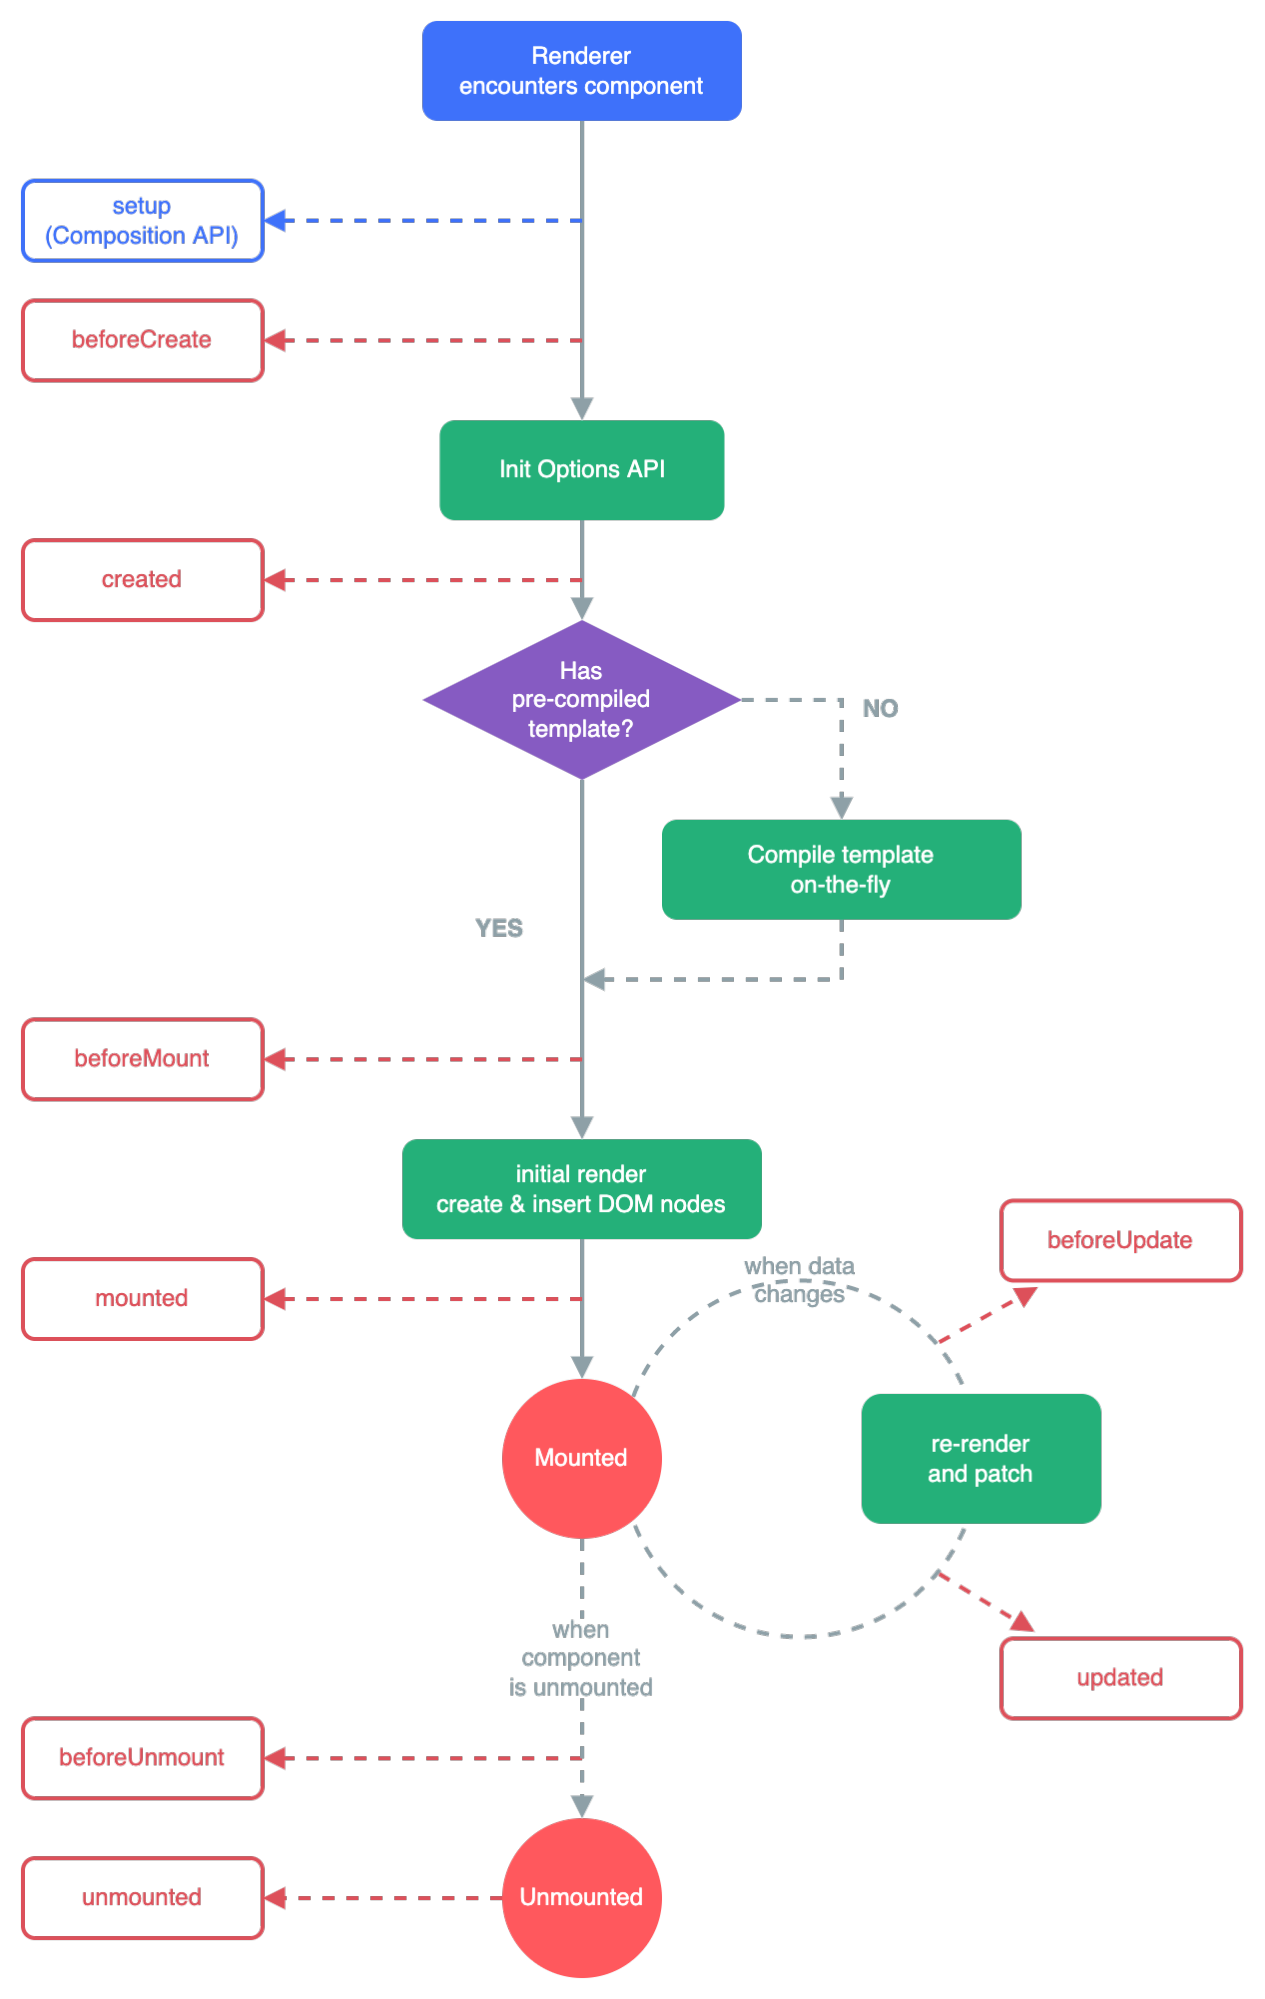
\includegraphics[width=10cm]{images/image09.png}
\end{center}

Lors de ces étapes de leur cycle, des fonctions peuvent être appelées pour effectuer des tâches. Ces fonctions sont appelées des {\color{monOrange}lifecycle hooks} (littéralement des accroches du cycle de vie).

Les {\color{monOrange}hooks} les plus utilisés sont :
\begin{itemize}
\item {\color{monOrange}onMounted()} : appelée juste après que le composant soit monté (donc lorsque le composant et ses descendants sont affichés sur le DOM).

\item {\color{monOrange}onUpdated()} : appelée lorsque le composant a été mis à jour et qu'un changement sur le DOM a été effectué.

\item {\color{monOrange}onUnmounted()} : appelée après que tous les effets réactifs aient été stoppés et lorsque le composant va être retiré du DOM. On l'utilise pour faire des opérations de nettoyage.
\end{itemize}
Les autres hooks sont :
\begin{itemize}
\item {\color{monOrange}onBeforeMount()} : qui est appelée lorsque le composant a été initialisé (notamment son état réactif) mais lorsqu'aucun élément n'a encore été créé sur le DOM.

\item {\color{monOrange}onBeforeUpdate()} : appelée juste avant que le composant n'ait mis à jour son DOM suite à un changement de son état réactif.

\item {\color{monOrange}onBeforeUnmount()} : appelée lorsque le composant est encore fonctionnel mais va être détruit.

\item {\color{monOrange}onErrorCaptured()} : appelée lorsqu'une erreur se propage depuis un composant enfant.

\end{itemize}

Nous verrons les autres {\color{monOrange}hooks} qui ont des cas avancés d'utilisations : {\color{monOrange} onRenderTracked(), onRenderTriggered(), onActivated(), onDeactivated() et onServerPrefetch()}. Ils sont relatifs au développement, aux composants {\color{monOrange}keepalive} et au {\color{monOrange}SSR}.

\subsection{Utiliser un {\color{monOrange}hook}}
Pour utiliser un hook c'est très simple, il suffit d'utiliser la fonction de {\color{monOrange}hook} adéquate et de lui passer une fonction de rappel contenant les tâches à exécuter lorsque l'état est atteint :
\begin{minted}[
mathescape,
framesep=2mm,
baselinestretch=1.2,
%fontsize=\footnotesize,
bgcolor=LightGray,
%linenos
]{html}
<script setup>
import { onMounted } from 'vue'

onMounted(() => {
  console.log('Le composant est présent sur le DOM.')
})
</script>
\end{minted}

%Exemple exécutable de la vidéo
%Vous pouvez directement utiliser ce code exécutable. N'hésitez pas à l'ouvrir dans un nouvel onglet pour le modifier ou mieux voir :

%%%%%%%%%%%%%%%%%%%%%%%%%%%%%%%%%%%%%%%%%%%%%%%%%%%%%%%%%%%%%%%%

\section{Les références de template}
\subsection{Les références de {\color{monOrange}templates}}
Parfois, vous voudrez accéder directement à un élément du DOM pour effectuer des opérations particulières. Dans ce cas, {\color{monOrange}Vue.js} propose de créer une référence côté {\color{monOrange}template} avec l'attribut {\color{monOrange}ref }:
\begin{minted}[
mathescape,
framesep=2mm,
baselinestretch=1.2,
%fontsize=\footnotesize,
bgcolor=LightGray,
%linenos
]{html}
<input ref="input">
\end{minted}
L'élément du DOM référencé devient alors accessible depuis le {\color{monOrange}script} :
\begin{minted}[
mathescape,
framesep=2mm,
baselinestretch=1.2,
%fontsize=\footnotesize,
bgcolor=LightGray,
%linenos
]{html}
<script setup>
import { ref, onMounted } from 'vue';

const input = ref(null);

onMounted(() => {
  input.value.focus();
})
</script>
\end{minted}
Le code précédent récupère le champ en utilisant la référence déclarée et va ensuite utiliser la méthode {\color{monOrange}focus()} permettant de cibler l'élément. Nous sommes sûr que le champ a été créé sur le DOM, car nous utilisons le {\color{monOrange}hook onMounted()} que nous avons vu dans la leçon précédente. Nous sommes obligé d'utiliser le {\color{monOrange}hook onMounted()} car nous manipulons un élément du DOM et il faut donc que celui-ci soit créé sur le DOM avant que nous y accédions.

\subsection{Utilisation des {\color{monOrange}refs} avec {\color{monOrange}v-for}}
Lorsque nous utilisons {\color{monOrange}ref} avec la directive {\color{monOrange}v-for}, il faut que la référence côté {\color{monOrange}script} contienne un tableau qui contiendra les éléments :
\begin{minted}[
mathescape,
framesep=2mm,
baselinestretch=1.2,
%fontsize=\footnotesize,
bgcolor=LightGray,
%linenos
]{html}
<script setup>
import { ref, onMounted } from 'vue';

const list = ref([1, 2, 3, 4]);

const itemRefs = ref([]);

onMounted(() => console.log(itemRefs.value));
</script>

<template>
  <ul>
    <li v-for="item in list" ref="itemRefs">
      {{ item }}
    </li>
  </ul>
</template>
\end{minted}

\subsection{Utilisation des {\color{monOrange}refs} avec des composants}
L'attribut {\color{monOrange}ref} peut également être utilisé sur les composants enfants. Par exemple :
\begin{minted}[
mathescape,
framesep=2mm,
baselinestretch=1.2,
%fontsize=\footnotesize,
bgcolor=LightGray,
%linenos
]{html}
<script setup>
import { ref, onMounted } from 'vue';
import Enfant from './Enfant.vue';

const enfant = ref(null);

onMounted(() => {
  // enfant.value contient l'élément Enfant
});
</script>

<template>
  <Enfant ref="enfant" />
</template>
\end{minted}
Attention ! Il n'est pas possible par défaut d'accéder aux propriétés des composants enfants en utilisant une référence car ces propriétés sont privées par défaut. Il faut exposer, avec {\color{monOrange}defineExpose()}, les propriétés auxquelles vous souhaitez accéder dans le composant parent, depuis le composant enfant :
\begin{minted}[
mathescape,
framesep=2mm,
baselinestretch=1.2,
%fontsize=\footnotesize,
bgcolor=LightGray,
%linenos
]{html}
<script setup>
import { ref } from 'vue';

const a = 21;
const b = ref(42);

defineExpose({
  a,
  b
})
</script>
\end{minted}
En utilisant {\color{monOrange}defineExpose()} nous rendons accessibles les deux variables depuis le composant parent qui peut ensuite les récupérer sur {\color{monOrange}enfant.value : enfant.value.a et enfant.value.b}.

\subsection{Utilisation de {\color{monOrange}TypeScript}}
Bien entendu, il faut également typer avec {\color{monOrange}TypeScript} les références. Nous allons voir comment le faire.

\subsubsection{Typer les références contenant des éléments HTML}
Les références doivent être typées avec une union de types entre {\color{monOrange}null} et le type d'élément HTML contenu dans la {\color{monOrange}ref}. Par exemple, pour un champ :
\begin{minted}[
mathescape,
framesep=2mm,
baselinestretch=1.2,
%fontsize=\footnotesize,
bgcolor=LightGray,
%linenos
]{html}
<script setup lang="ts">
import { ref, onMounted } from 'vue';

const el = ref<HTMLInputElement | null>(null);

onMounted(() => {
  el.value?.focus();
});
</script>

<template>
  <input ref="el" />
</template>
\end{minted}
Ici nous passons en type générique {\tt <HTMLInputElement | null>} à {\color{monOrange}ref()} pour lui indiquer que la référence peut être null (lorsque l'élément n'est pas encore sur le DOM) ou alors un élément de type {\color{monOrange}HTMLInputElement}. Notez également qu'il faut indiquer que la référence est null lors de l'initialisation du composant en passant null comme valeur initiale à {\color{monOrange}ref()}.

{\em L'opérateur de chaînage optionnel ?. est un opérateur JavaScript qui permet de lire la valeur d'une propriété sans avoir à valider expressément que chaque référence dans la chaîne n'est ni {\color{monOrange}null} ni {\color{monOrange}undefined}.}

Ici nous avons besoin d'utiliser cet opérateur car {\color{monOrange}el} est {\color{monOrange}null} avant le montage du composant sur le DOM. La référence peut également être null dans d'autres cas, par exemple en utilisant la directive {\color{monOrange}v-if} et si la condition n'est pas remplie.

\subsubsection{Typer les références contenant des composants}
Pour les composants, il faut typer de cette manière :
\begin{minted}[
mathescape,
framesep=2mm,
baselinestretch=1.2,
%fontsize=\footnotesize,
bgcolor=LightGray,
%linenos
]{html}
<script setup lang="ts">
import Enfant from './Enfant.vue';

const modal = ref<InstanceType<typeof Enfant> | null>(null);

const openModal = () => {
  modal.value?.open();
};
</script>
\end{minted}
\begin{itemize}
\item {\tt typeof }: permet de récupérer le type d'un élément, ici le type du composant enfant.

\item {\tt InstanceType} : permet de créer un type à partir d'un type d'une instance de fonction constructrice.

\item {\tt ref<InstanceType<typeof Enfant> | null>} : nous récupérons l'instance du composant, récupérons son type avec {\color{monOrange}typeof}, construisons le type de la fonction constructrice du composant à partir de cette instance du composant. Nous indiquons également que la référence peut être {\color{monOrange}null}.

\end{itemize}
%Exemple exécutable de la vidéo
%Vous pouvez directement utiliser ce code exécutable. N'hésitez pas à l'ouvrir dans un nouvel onglet pour le modifier ou mieux voir :

%%%%%%%%%%%%%%%%%%%%%%%%%%%%%%%%%%%%%%%%%%%%%%%%%%%%%%%%%%%

\section{Utilisation des liaisons et des directives sur les composants}
\subsection{Utilisation des classes sur les composants}
Lorsque vous utilisez l'attribut {\color{monOrange}class} avec un composant enfant, ces classes seront ajoutées sur l'élément racine, c'est-à-dire l'élément imbriquant tous les autres éléments du {\color{monOrange}template} du composant enfant. Par exemple, si le composant enfant a pour {\color{monOrange}template} :
\begin{minted}[
mathescape,
framesep=2mm,
baselinestretch=1.2,
%fontsize=\footnotesize,
bgcolor=LightGray,
%linenos
]{html}
<div class="classe1">
  <p>Bonjour !</p>
</div>
\end{minted}
Et que nous utilisons l'attribut {\color{monOrange}class} dans le {\color{monOrange}template} du composant parent, sur le composant enfant :
\begin{minted}[
mathescape,
framesep=2mm,
baselinestretch=1.2,
%fontsize=\footnotesize,
bgcolor=LightGray,
%linenos
]{html}
<Enfant class="classe2" />
\end{minted}
{\color{monOrange}Vue.js} résolvera les classes en les fusionnant :
\begin{minted}[
mathescape,
framesep=2mm,
baselinestretch=1.2,
%fontsize=\footnotesize,
bgcolor=LightGray,
%linenos
]{html}
<div class="classe1 classe2">
  <p>Bonjour !</p>
</div>
\end{minted}
Attention ! Si le composant enfant n'a pas d'élément racine imbriquant les autres éléments du {\color{monOrange}template}, il faudra utiliser la valeur spéciale {\color{monOrange}\$attrs.class} mise à disposition par {\color{monOrange}Vue.js}. Ainsi, nous devrons faire :
\begin{minted}[
mathescape,
framesep=2mm,
baselinestretch=1.2,
%fontsize=\footnotesize,
bgcolor=LightGray,
%linenos
]{html}
<p :class="$attrs.class">Bonjour </p>
<span>C'est le template du composant enfant</span>
\end{minted}
Ici nous disons à {\color{monOrange}Vue.js} d'appliquer les classes définies dans le composant parent sur l'élément paragraphe. C'est tout à fait logique : {\color{monOrange}Vue.js} ne sait pas où appliquer les classes si nous ne lui indiquons pas, et donc par défaut il ne va rien appliquer.

\subsection{Utilisation de la directive {\color{monOrange}v-for} avec des composants}
La directive {\color{monOrange}v-for} est utilisable directement sur tout composant :
\begin{minted}[
mathescape,
framesep=2mm,
baselinestretch=1.2,
%fontsize=\footnotesize,
bgcolor=LightGray,
%linenos
]{html}
<Composant v-for="item in items" :key="item.id" />
\end{minted}
Pour passer des données au composant enfant, il faut utiliser la liaison de données avec {\color{monOrange}v-bind} :
\begin{minted}[
mathescape,
framesep=2mm,
baselinestretch=1.2,
%fontsize=\footnotesize,
bgcolor=LightGray,
%linenos
]{html}
<Composant v-for="(item, index) in items" :item="item" :index="index" :key="item.id"  />
\end{minted}

\subsection{Utilisation de la directive {\color{monOrange}v-if} avec des composants}
Il n'y a rien de particulier pour la directive {\color{monOrange}v-if} que vous pouvez appliquer sur tous les composants :
\begin{minted}[
mathescape,
framesep=2mm,
baselinestretch=1.2,
%fontsize=\footnotesize,
bgcolor=LightGray,
%linenos
]{html}
<Composant v-if="active" />
\end{minted}

%Exemple exécutable de la vidéo
%Vous pouvez directement utiliser ce code exécutable. N'hésitez pas à l'ouvrir dans un nouvel onglet pour le modifier ou mieux voir :
